\documentclass[10pt, xcolor=x11names]{beamer}
\usecolortheme{seagull}
\useoutertheme{infolines}
\usefonttheme[onlymath]{serif}
\setbeamertemplate{headline}[default]
\setbeamertemplate{navigation symbols}{}
\mode<beamer>{\setbeamertemplate{blocks}[rounded][shadow=true]}
\setbeamercovered{transparent}
\setbeamercolor{block body example}{fg=blue, bg=black!20}

\usepackage[utf8]{inputenc}
\usepackage[german]{babel}
\usepackage[]{csquotes}
\usepackage{amsmath}
\usepackage{tikz, wasysym}
\usepackage{graphicx}
\usetikzlibrary{automata,positioning}
\usepackage{hyperref}

\usepackage[]{algorithm2e}
%\usepackage{amsfonts}
%\usepackage{amssymb}
%\usepackage{makeidx}
%\usepackage{graphicx}


\usepackage{hyperref}
\author{Sven Fiergolla}
\title[Großes Studienprojekt]{Index Creation}
\subtitle[short version]{}
\date{\today}
%\institute[Uni Trier]{Universität Trier}
%\logo{\includegraphics[scale=.25]{unilogo.pdf}}

\begin{document}
	\frame{\maketitle}
	\frame{\frametitle{Übersicht}
	\tableofcontents
	}
	

	\section{Einführung}
	\frame{\frametitle{Einführung}

	Effiziente Suche über:
	\bigskip
	\begin{description}
	\item Sammlung von Büchern
	\item das Web
	\item andere große Datenmengen
\end{description}
\bigskip
\pause zu viel für Main Memory!

	}	
	
	\frame{\frametitle{Einführung}
Typische Systemeigenschaften (stand 2018)
\medskip
\begin{itemize}
	\item \textit{clock rate} 2-4 GHz, 4-8 Kerne
	\item \textit{main memory} 4-32 GHz
	\item \textit{disk space} $\leq$ 1 TB SSD oder $\geq$ 1 TB HDD
	\pause 
	\begin{itemize}
	\item HDD (hard disk drive)
	\begin{itemize}
	\item \textit{average seek time} zwischen 2 und 20 ms
	\item \textit{transfer time} 150 - 300 MB/s
	\end{itemize}
	\pause \item SSD (solid state disk)
	\begin{itemize}
	\item \textit{average seek time} zwischen 0.08 und 0.16 ms
	\item \textit{transfer time} Lesen: 545 MB/s, Schreiben: 525 MB/s
	\end{itemize}
	\end{itemize}
\end{itemize}	
}



	
	
	\section{Hardware constraints}	
		\frame{\frametitle{hardware constraints}
		Indizierung einer Sammlung von Daten auf der Festplatte\\
		\bigskip
		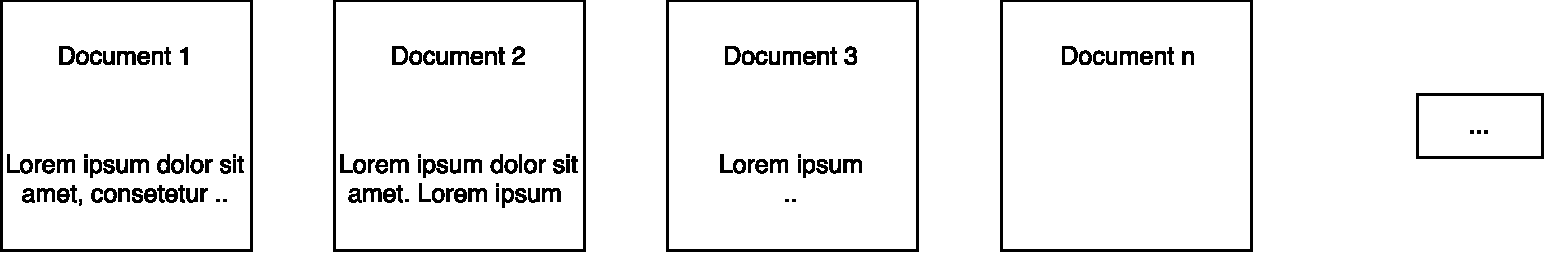
\includegraphics[scale=0.4]{pdf/Documents.pdf}\\
		\bigskip
		Zugriffszeit auf Festplatte als Bottelneck
	}	
	
	

	\section{Index Creation}
	\frame{\frametitle{Index Creation}
	geeignete Datenstruktur um Zugriff auf die Festplatte zu minimieren
	\bigskip
\only<1>{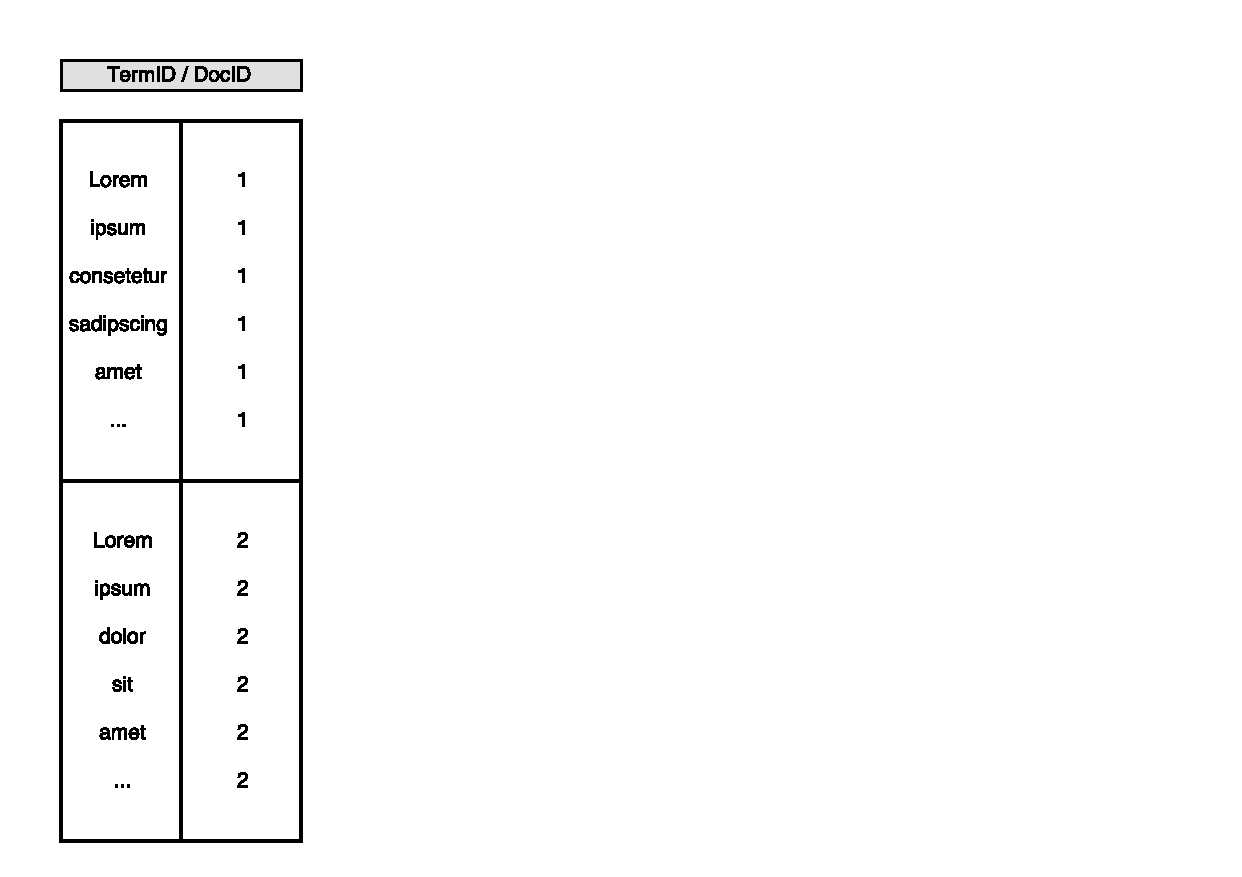
\includegraphics[scale=0.55]{pdf/postingslist1.pdf}}
\only<2>{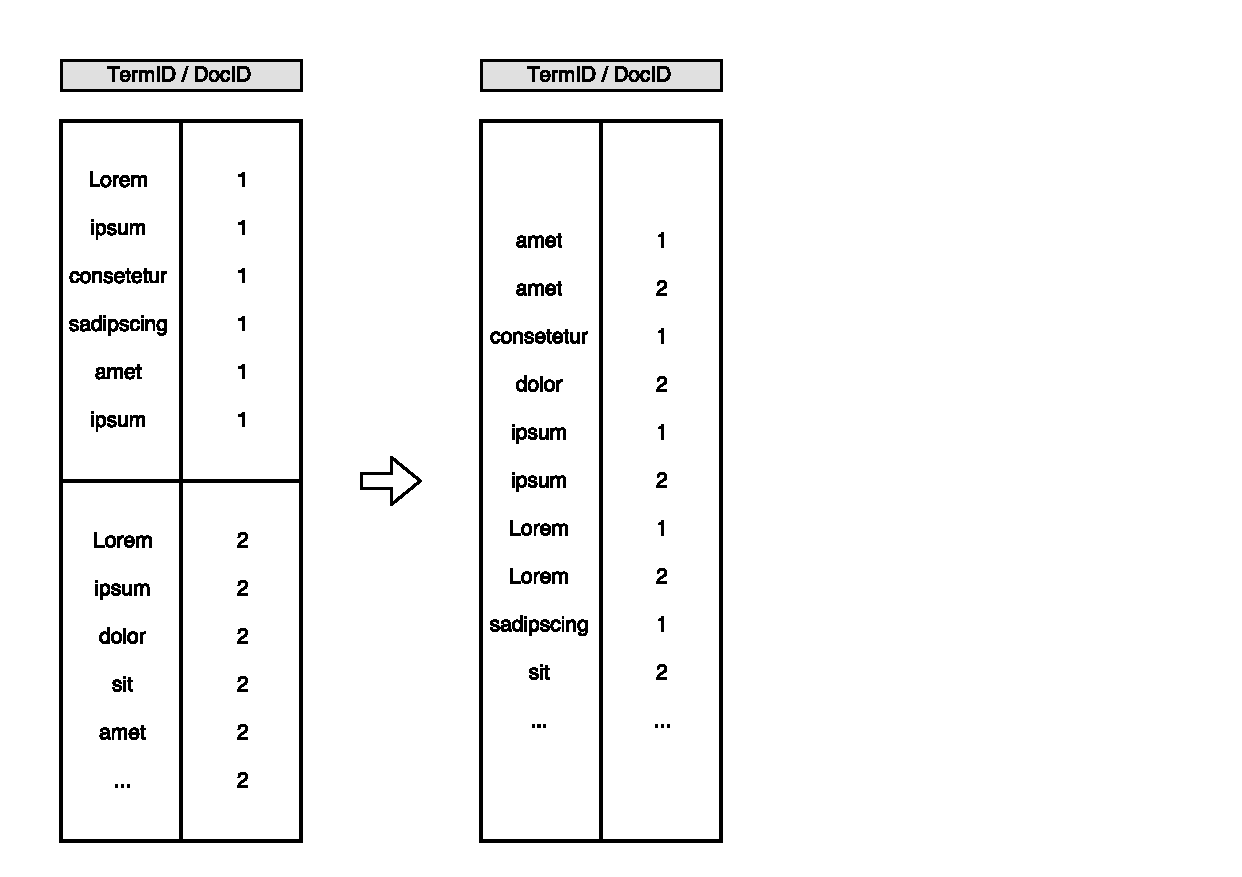
\includegraphics[scale=0.55]{pdf/postingslist2.pdf}}
\only<3>{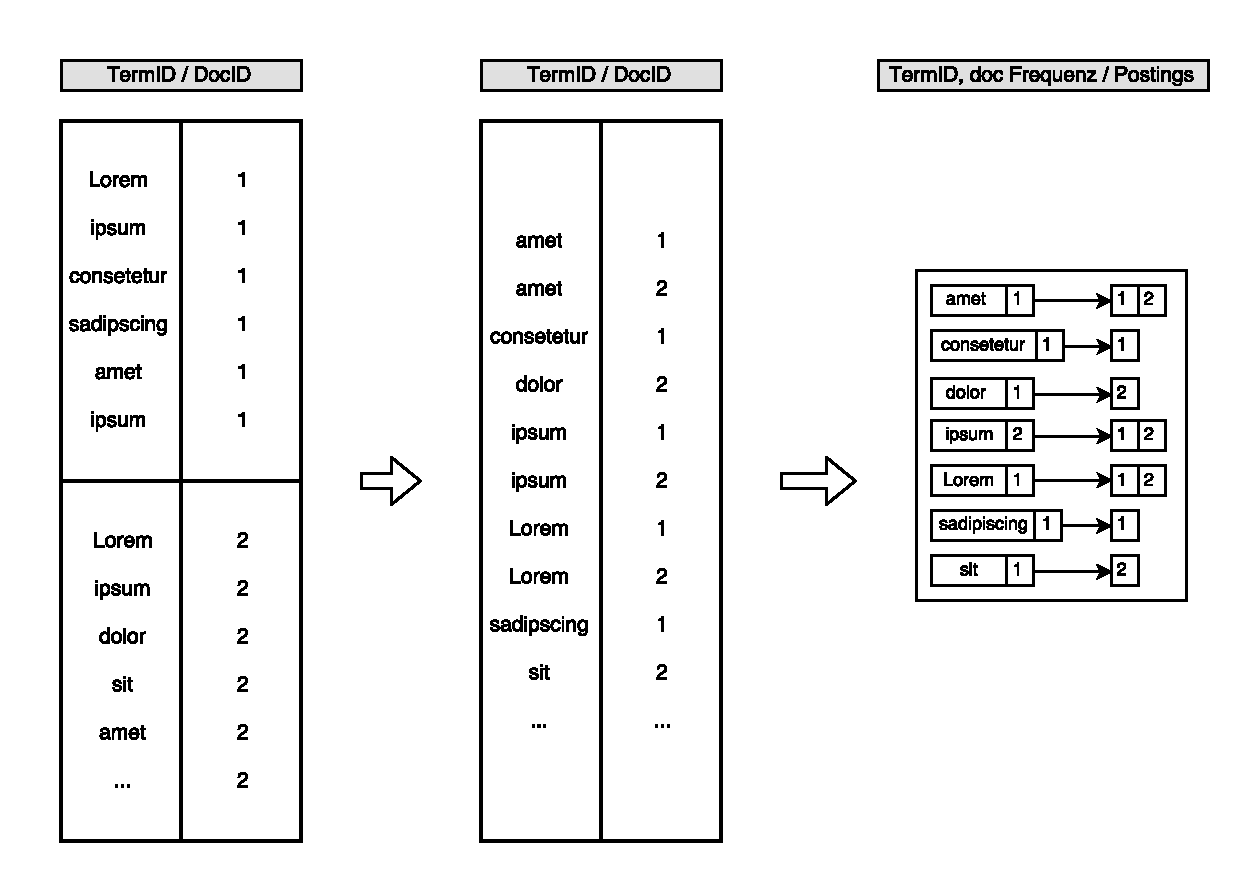
\includegraphics[scale=0.55]{pdf/postingslist3.pdf}}

}

\subsection{Blocked sort-based indexing}
	 	\frame{\frametitle{Index Creation - hardware constraints}
		in der Regel übersteigt die Datenmenge der Dokumente den Main Memory.\\
		\bigskip
		\bigskip
		Reuters-RCV1 benötigt ca 0.8 GB für die termID/DocID Paare, bereits die DBLP übersteigt die Dokumentenanzahl, besitzt jedoch weniger Terme.
	}

		\frame{\frametitle{Blocked sort-based indexing (BSI)}
\begin{columns}
    \begin{column}{0.47\textwidth}
	Lösung:\\
	\begin{itemize}
	\item Sammlung von Dokumenten in einzelne Blocks unterteilen
	\item Index über einzelne Blöcke erstellen
	\item Teilindizes mergen
	\end{itemize}
\end{column}
 \begin{column}{0.47\textwidth}
\begin{algorithm}[H]
\caption{BSI Algorithmus}
 n = 0\;
 \While{all documents have not been processed}{
n = n + 1\;
block = ParseNextBlock()\;
BSBI-INVERT(block)\;
WriteBlockToDisk(block, $f_n$)\;
  }
  MergeBlocks($f_1$, $\cdots$, $f_n$; $f_{merged}$)\;
\end{algorithm}
\end{column}
\end{columns}
}
	
		\frame{\frametitle{Blocked sort-based indexing (BSI) - merging Blocks}
\only<1>{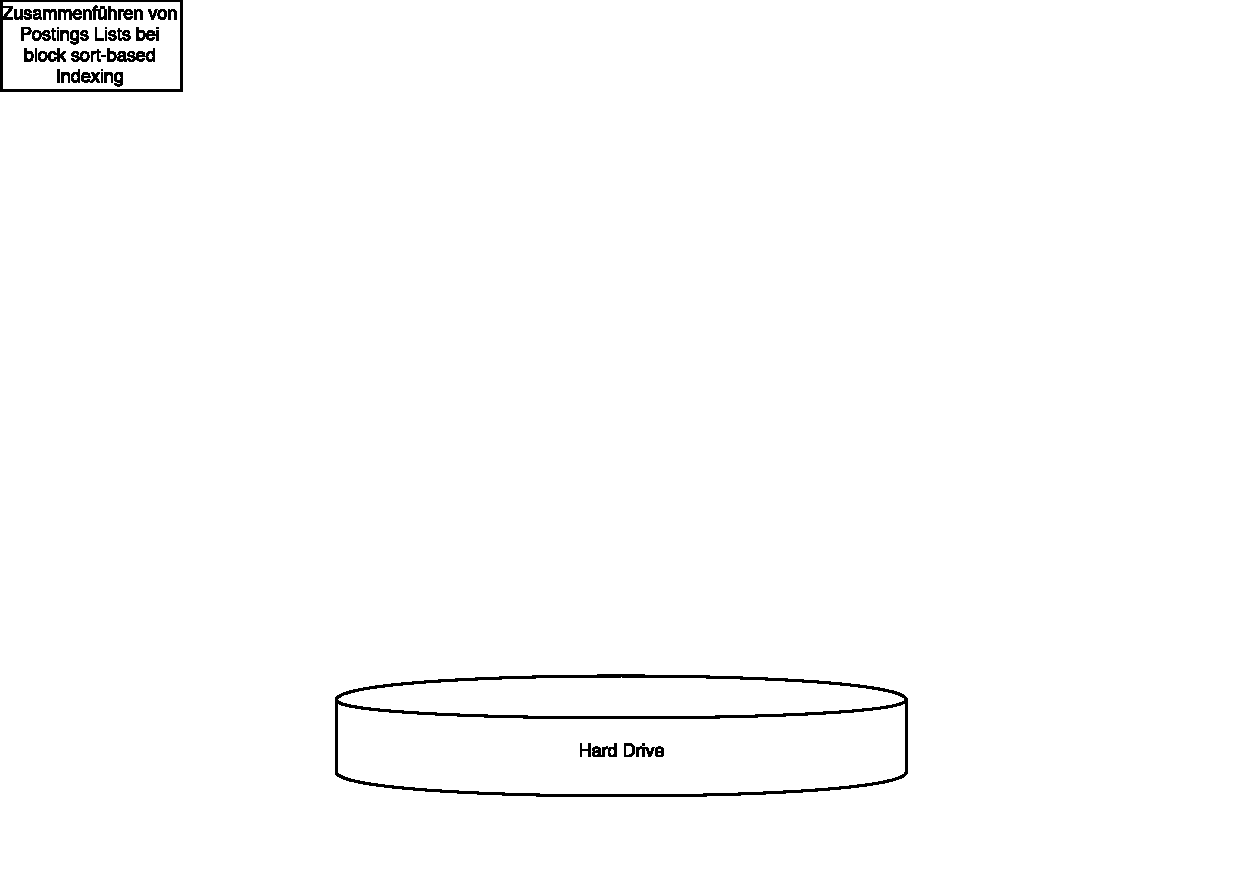
\includegraphics[scale=0.55]{pdf/BSI_merging1.pdf}}
\only<2>{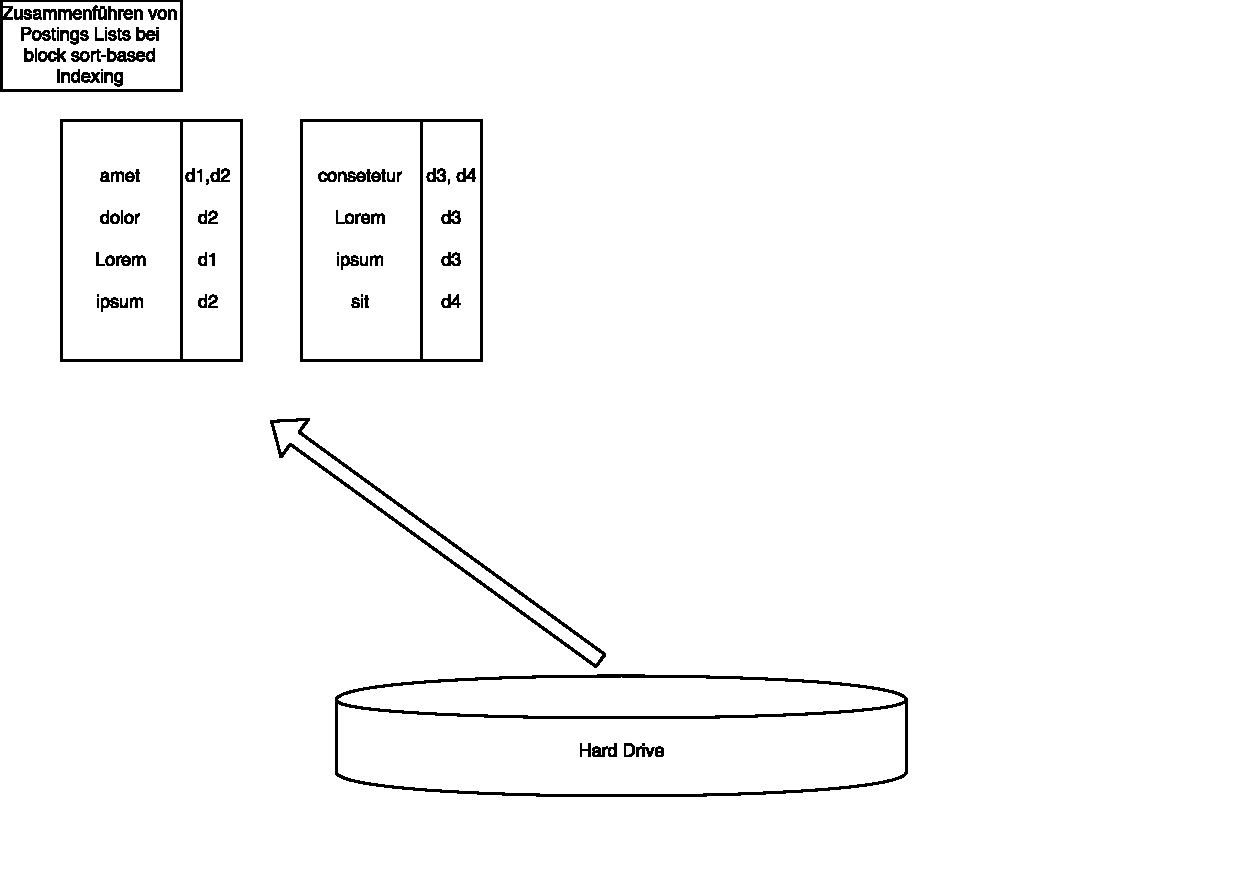
\includegraphics[scale=0.55]{pdf/BSI_merging2.pdf}}
\only<3>{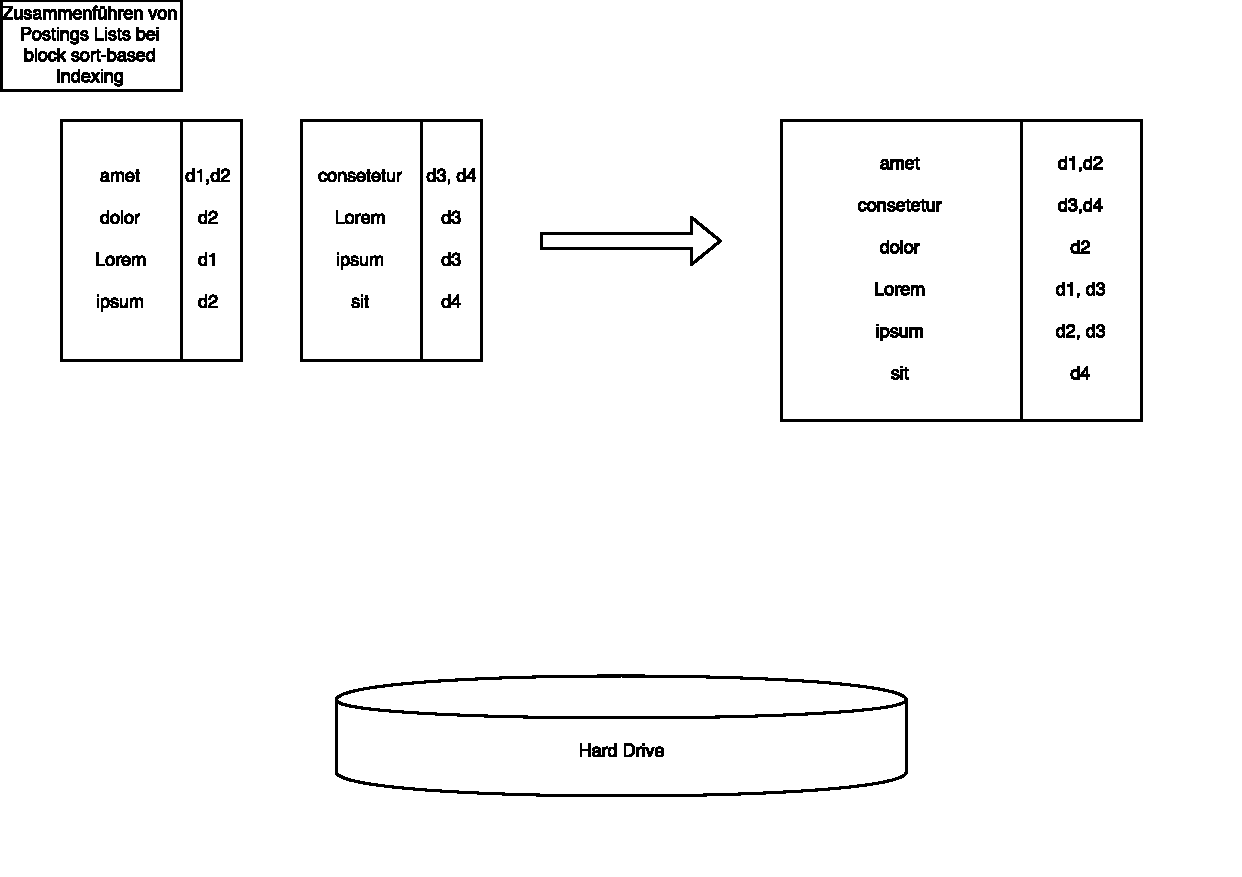
\includegraphics[scale=0.55]{pdf/BSI_merging3.pdf}}
\only<4>{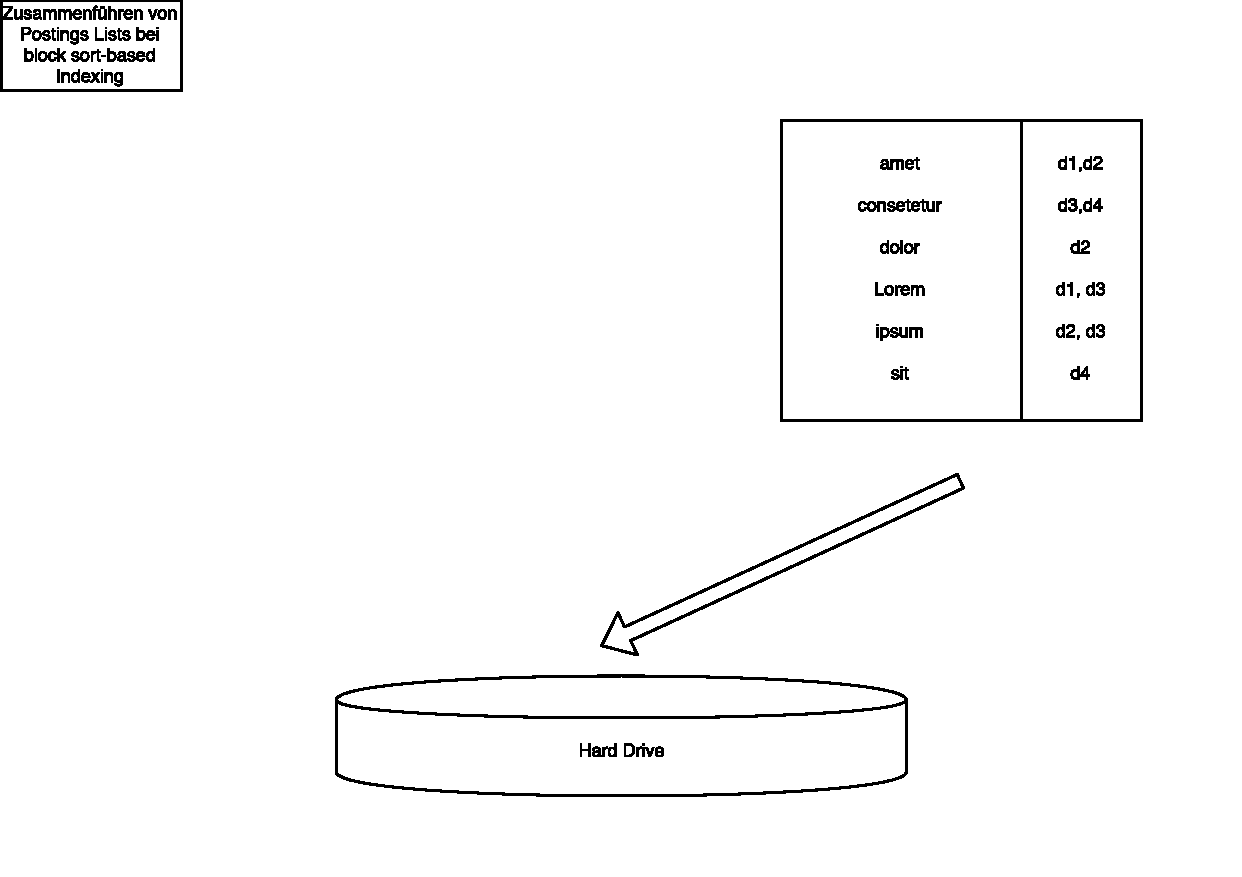
\includegraphics[scale=0.55]{pdf/BSI_merging4.pdf}}
}

			\frame{\frametitle{Blocked sort-based indexing (BSI) - Fazit}
			Fazit zu BSBI:
			\begin{itemize}
			\item Zeitkompplexität:	$\Theta ( T \cdot log(T))$
			\begin{itemize}
			\item das Sortieren hat die höchste Komplexität
			\item das Parsen und Mergen der Blocks ist jedoch in der Regel am Zeitaufwendigsten
			\end{itemize}
			\item Datenstruktur für Mapping zwischen termen und termID's muss in Main Memory liegen
			\begin{itemize}
			\item kann für sehr große Datenmengen auch Server überlasten
			\end{itemize}
			\end{itemize}

}




	
\subsection{Single-pass in-memory indexing}
			\frame{\frametitle{Single-pass in-memory indexing (SPIMI)}
\begin{itemize}
\item einzelne dictionaries für jeden Block
\begin{itemize}
\item keine Datenstruktur für das Mapping von termen und termID's
\end{itemize}
\item kein Sortieren der einzelnen Blöcke
\begin{itemize}
\item Postings in der Reihenfolge ihres Vorkommens in die Postingslist aufnehmen
\item PostingsList sollte jedoch sortiert werden, da dann auf Sortieren/Suchen beim mergen der Blöcke verzichtet werden kann
\end{itemize}

\end{itemize}			
}

			\frame{\frametitle{Single-pass in-memory indexing (SPIMI)}
SPIMI-invert(TokenStream)
\begin{algorithm}[H]
\caption{SPIMI-invert Algorithmus}
 outputFile = new HashFile()\;
 dictionary = new HashFile()\;
 \While{free memory available}{
 token = next(TokenStream)\;
\eIf{term(token) $\notin$ dictionary}{
PostingsList = AddToDictionary(dictionary, term(token))\;
}{
PostingsList = GetPostingsList(dictionary, term(token))\;
}
\If{full(PostingsList)}{
PostingsList = DoublePostingsList(dictionary, term(token))\;
}
AddToPostingsList(PostingsList, docID(token))\;
SortedTerms = SortTerms(dictionary)\;
WriteBlockToDisk(SortedTerms, dictionary, OutputFile)\;
  }
\end{algorithm}
}

\frame{\frametitle{Single-pass in-memory indexing (SPIMI)}
Vorteile gegenüber BSI:
\begin{itemize}
\item kann für beliebig große Datenmengen einen Index erstellen, solange das Festplattenvolumen nicht überstiegen wird
\item einzelne Blocke können größer sein
\begin{itemize}
\item Indexerstelung effizienter
\end{itemize}
\item distionaries und die erstellte PostingsList kann durch Kompression kompakt auf der Festplatte gespeichert werden
\end{itemize}
}


\subsection{Distributed indexing}
\frame{\frametitle{Distributed indexing}
\begin{columns}
\begin{column}{0.47\textwidth}
\begin{itemize}
\item manche Sammlungen übersteigen die Leistung eines einzelnen Rechners
\begin{itemize}
\item beispielsweise das Web
\end{itemize}
\item um Indizes über solche Sammlungen zu erstellen, muss die Arbeit auf mehrere Rechner verteilt werden
\end{itemize}
\end{column}
\begin{column}{0.47\textwidth}
\only<2>{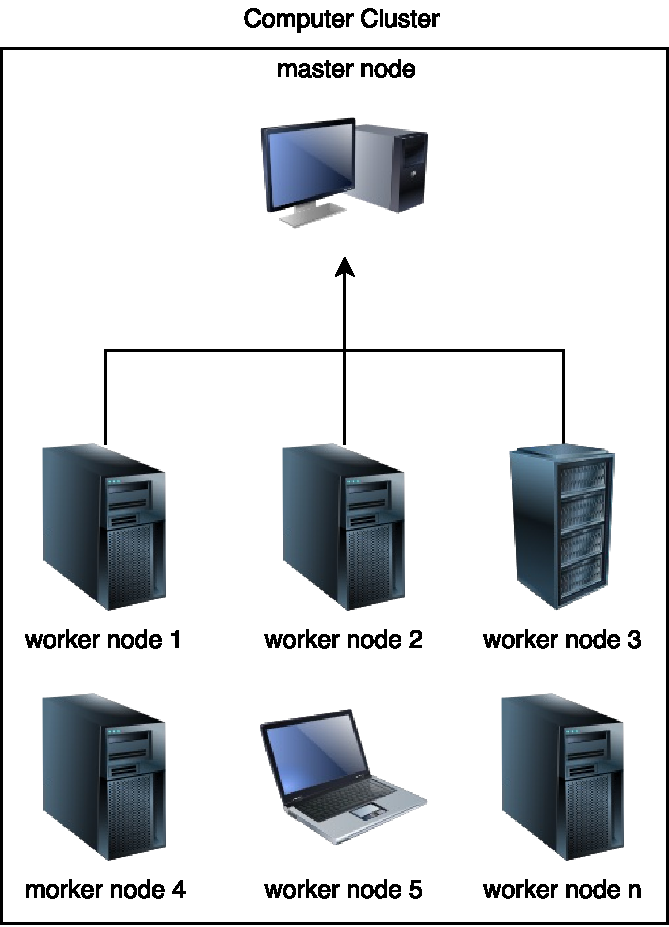
\includegraphics[scale=0.4]{pdf/mapreduce.pdf}}
\end{column}
\end{columns}
}
\frame{\frametitle{Distributed indexing - MapReduce}
\only<1>{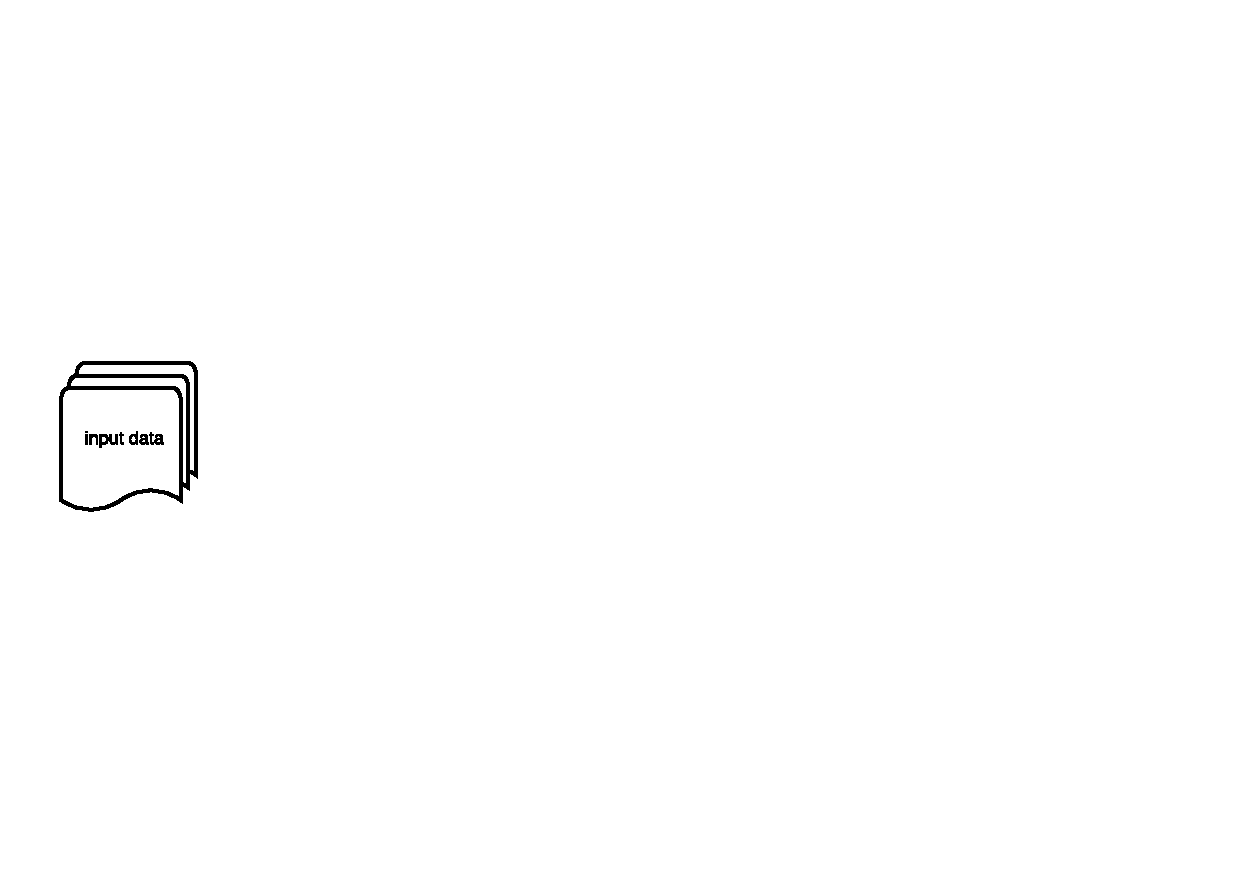
\includegraphics[scale=0.55]{pdf/distributedIndex.pdf}}
\only<2>{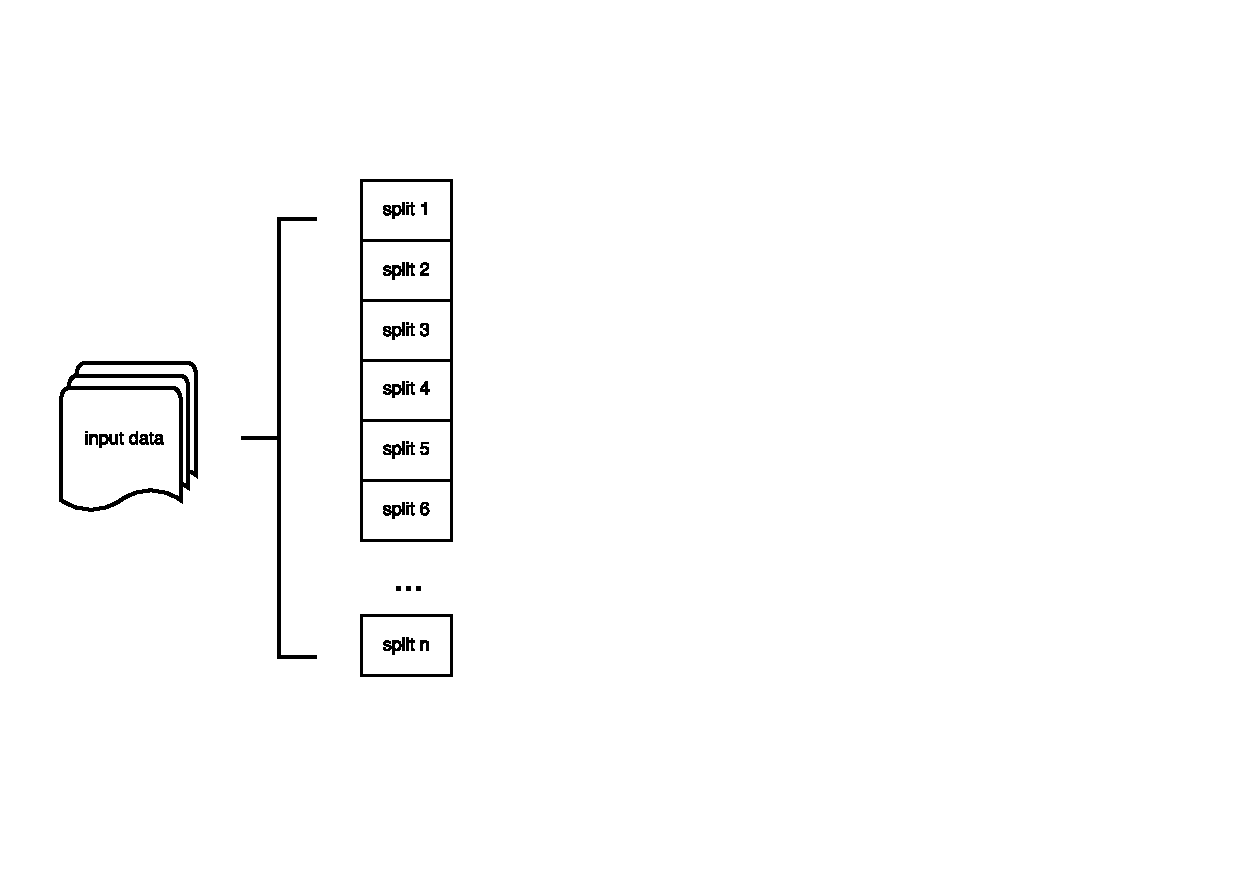
\includegraphics[scale=0.55]{pdf/distributedIndex2.pdf}}
\only<3>{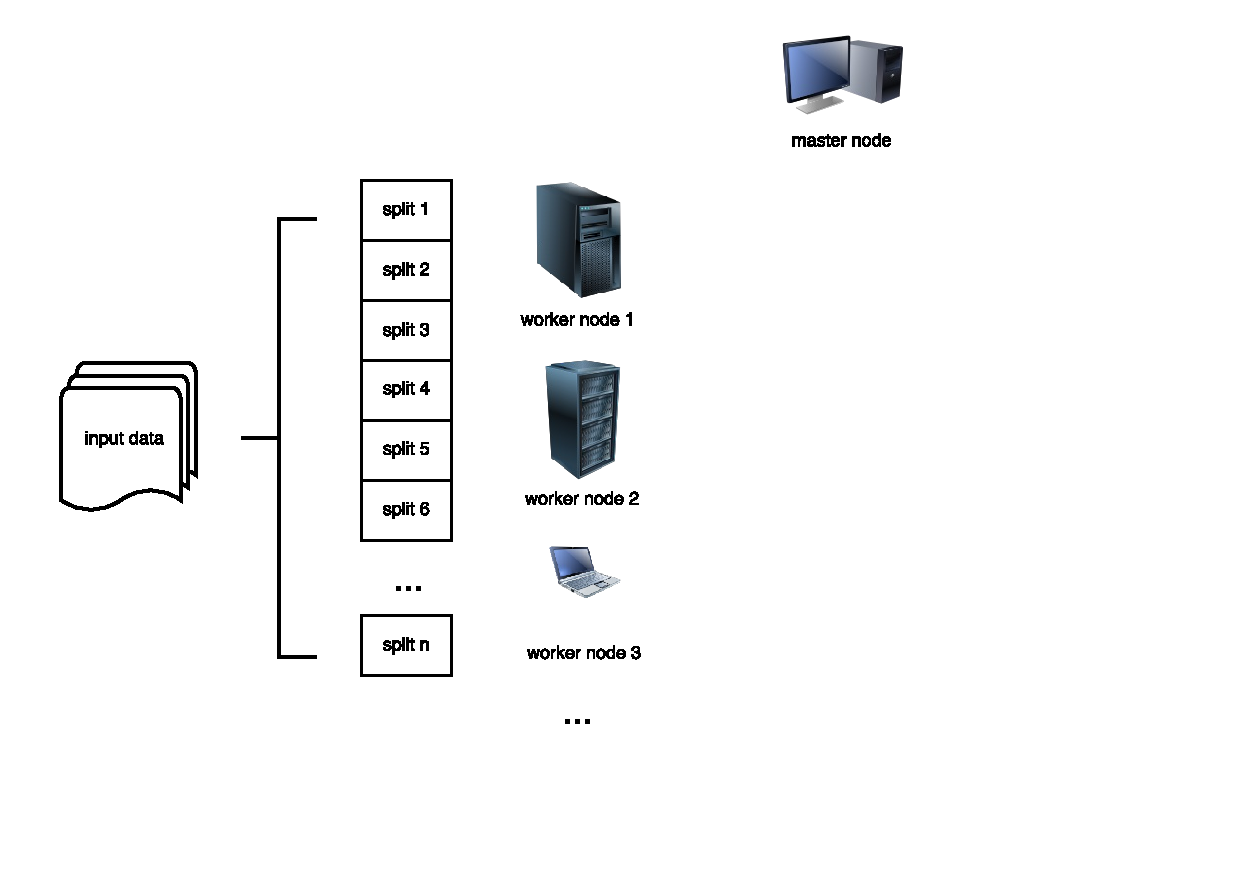
\includegraphics[scale=0.55]{pdf/distributedIndex3.pdf}}
\only<4>{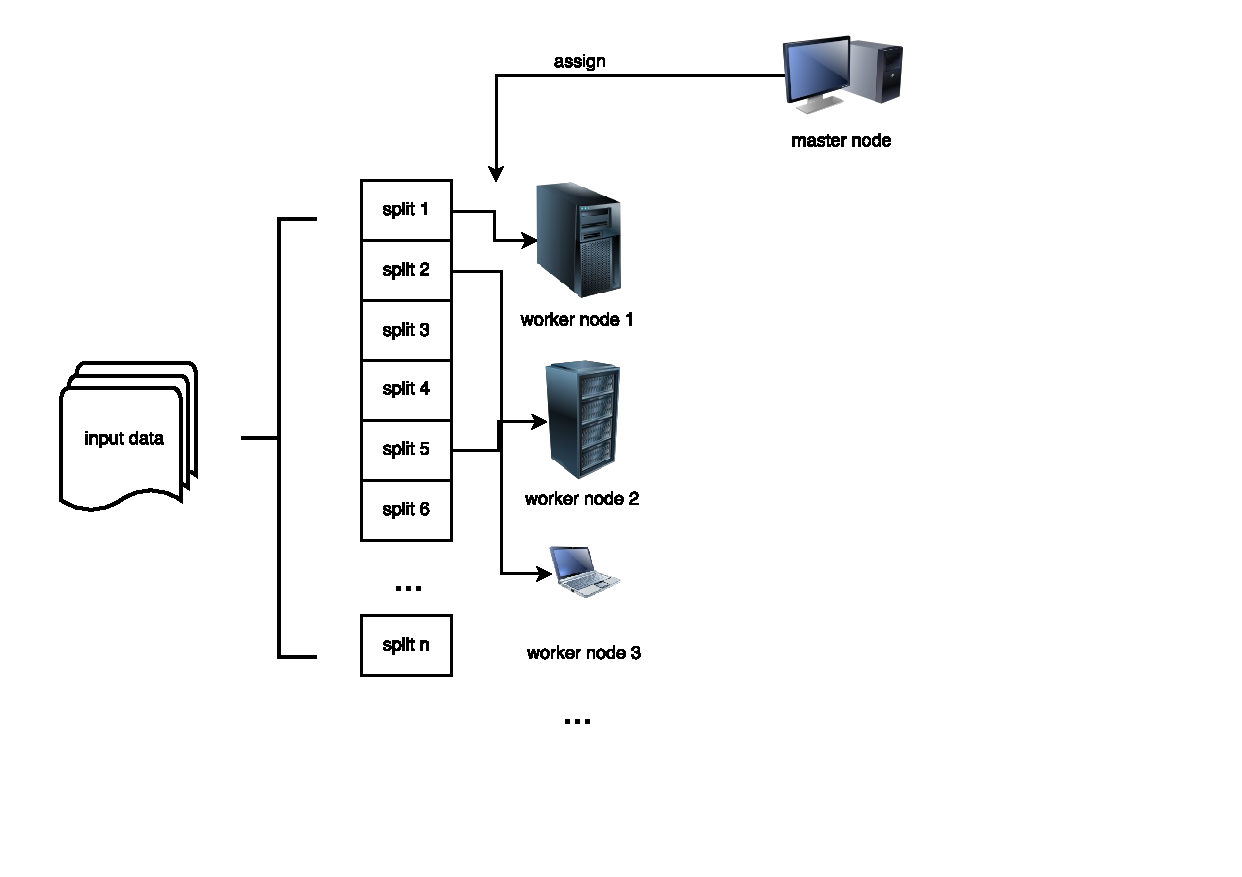
\includegraphics[scale=0.55]{pdf/distributedIndex4.pdf}}
\only<5>{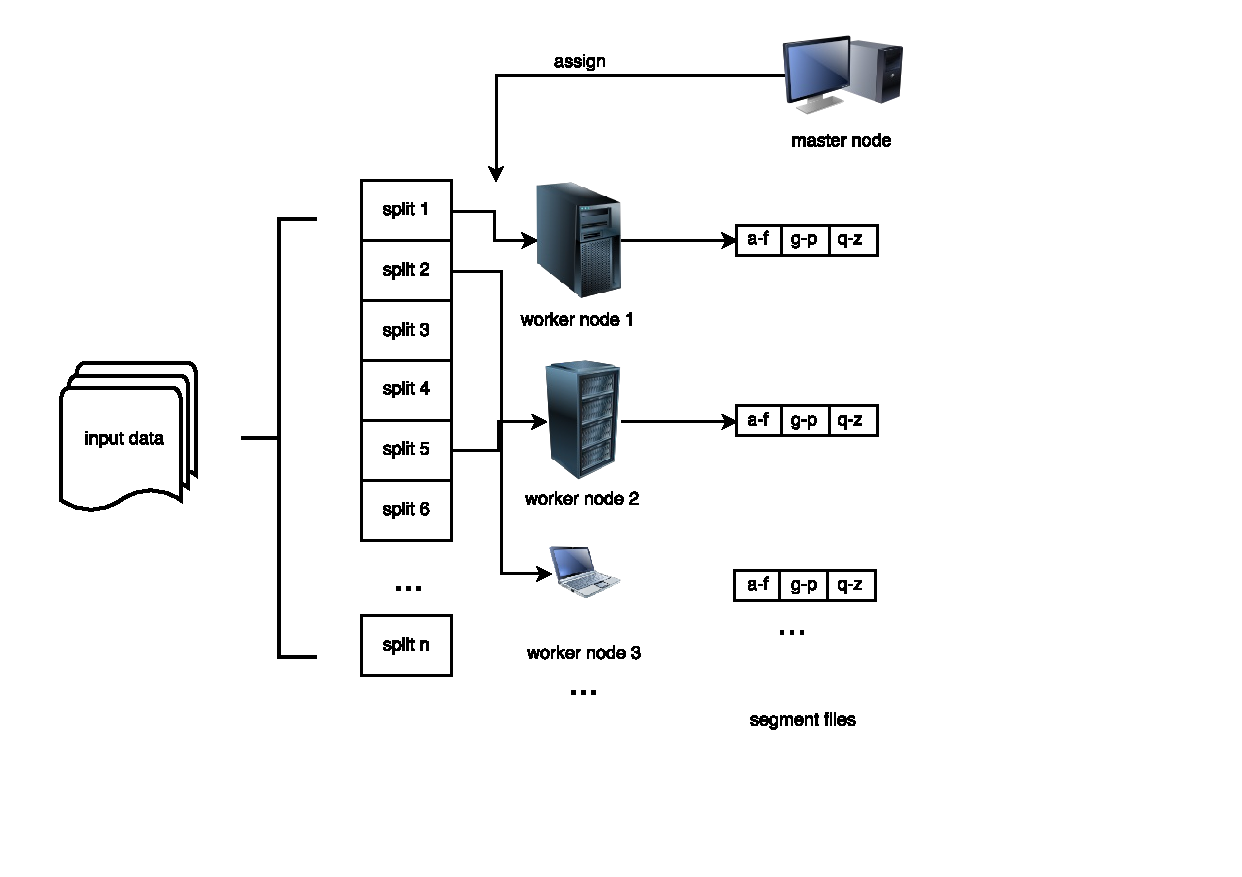
\includegraphics[scale=0.55]{pdf/distributedIndex5.pdf}}
\only<6>{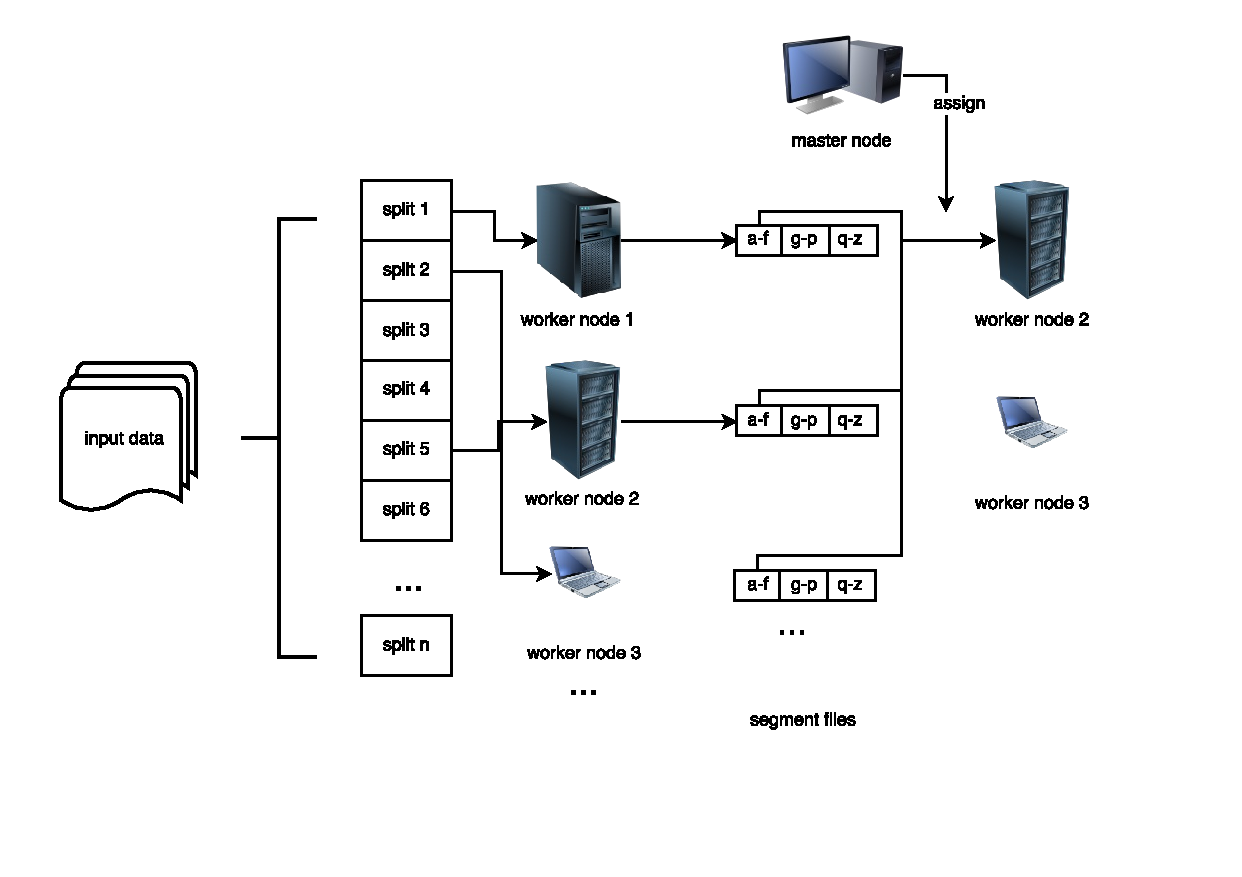
\includegraphics[scale=0.55]{pdf/distributedIndex6.pdf}}
\only<7>{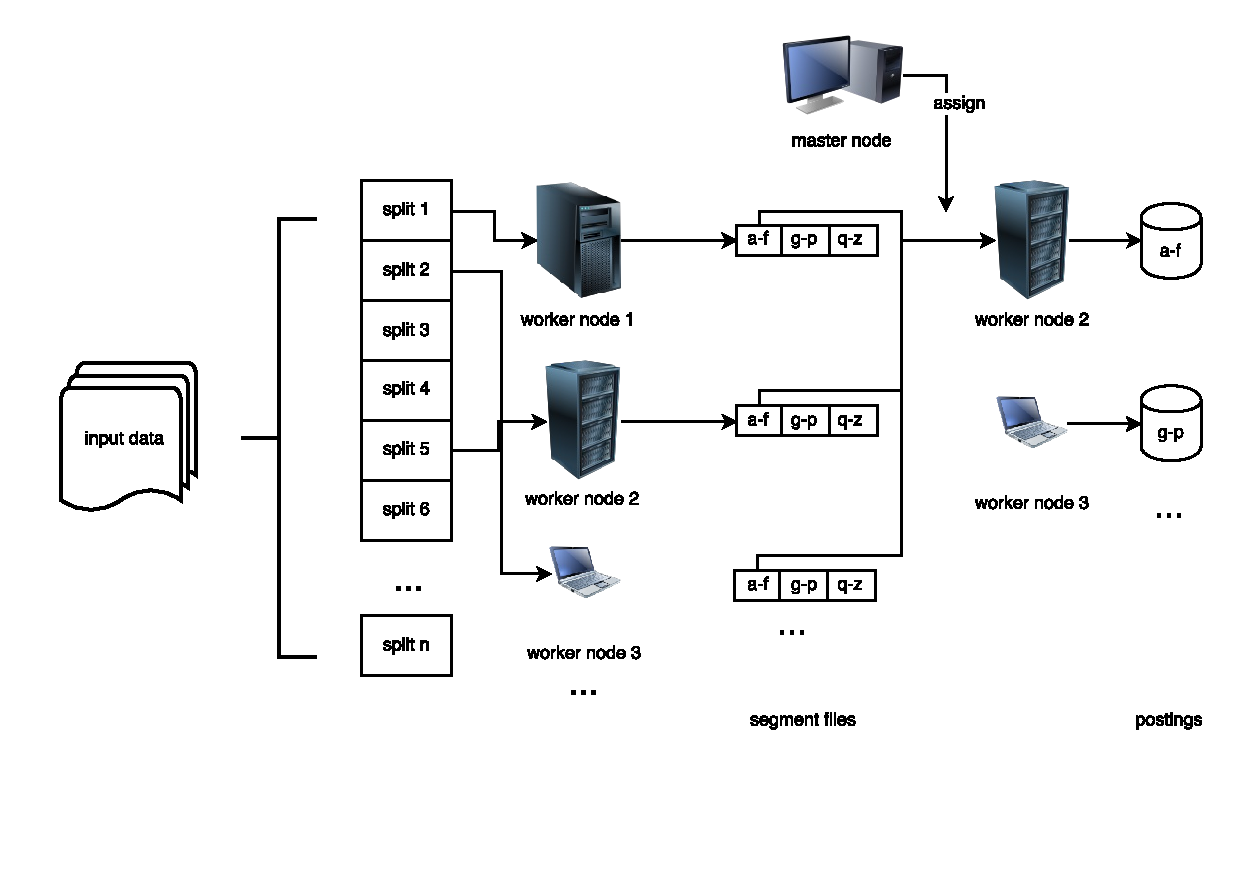
\includegraphics[scale=0.55]{pdf/distributedIndex7.pdf}}
}

\frame{\frametitle{Distributed indexing - Fazit}
todo}

\subsection{Dynamic indexing}
\frame{\frametitle{Dynamic indexing}
\begin{itemize}
\item viele Sammlungen von Dokumenten ändern sich häufig
\begin{itemize}
\item beispielsweise werden Webseiten geändert, gelöscht oder neue hinzugefügt
\end{itemize}
\item daher muss die Indexerstellung über eine solche Sammlung ebenfalls dynamsich sein
\end{itemize}
}

\subsection{andere Indexierungsverfahren}

\section{Indexierung mit Solid State Drives}

\section{Fazit}

\section{Quellen}
	 	 \frame{\frametitle{Quellen}
	
	\begin{itemize}
		\item Christopher D. Manning, Prabhakar Raghavan and Hinrich Schütze \enquote{Introduction to Information Retrieval} \footnote{\url{https://nlp.stanford.edu/IR-book/pdf/04const.pdf}} Cambridge University Press 2008, pp. 1-18 and 67-84.

	 \item Ian H. Witten, Alistair Moffat, Timothy C. Bell \enquote{Managing Gigabytes: Compressing and Indexing Documents and Images}  \footnote{\url{https://books.google.de/books?id=2F74jyPl48EC&dq=Witten+et+al.+index+1999&lr=&hl=de&source=gbs_navlinks_s}} Morgan Kaufman Publishers 1999, pp. 223-261.
	 
	\item Stephen M Ash, King-Ip Lin (University of Memphis) \enquote{Optimizing Database Index Performance for Solid State Drives} \footnote{\url{http://cs.baylor.edu/~lind/_mypaper/ashlin.pdf}} IDEAS ’14, July 07 - 09 2014, Porrto, Portugal.
	
	\item Yinan Li, Bingsheng He, Robin Jun Yang, Qiong Luo, Ke YiTree (Hong Kong University of Science and Technology) \enquote{Indexing on Solid State Drives} \footnote{\url{http://pages.cs.wisc.edu/~yinan/paper/fdtree_pvldb.pdf}} The 36th International Conference on Very Large Data Bases, September 13-17,
2010, Singapore.
	 
\end{itemize}
	 }
	
	
	
\end{document}
